\documentclass{article}
\usepackage{enumerate}
\usepackage{amsmath}
\usepackage{amssymb}
\usepackage{graphicx}
\usepackage{subfigure}
\usepackage{geometry}
\usepackage{caption}
\usepackage{indentfirst}
\usepackage{tikz}
\usetikzlibrary{circuits.logic.US}
\usetikzlibrary{arrows.meta}
\usetikzlibrary{calc}
\geometry{left=3.0cm,right=3.0cm,top=3.0cm,bottom=3.0cm}
\renewcommand{\thesection}{Problem \arabic{section}.}
\title{VE270 Homework 9}
\author{Liu Yihao 515370910207}
\date{}

\begin{document}
\maketitle

\newcommand{\drawadder}[4]{
	\draw #1 node (#2) [shape=rectangle,draw,minimum height=2cm,minimum width=3cm,text width=3cm,align=center] {#3};
	\draw (#2) ++(down:7.5mm) node {$s$};
	\draw (#2) ++(up:7.5mm) ++(left:5mm) node {$a$} ++(right:10mm) node {$b$};
	\draw (#2) ++(down:10mm) to node {$\diagup$} node[left] {#4} ++(down:5mm) ;
	\draw (#2) ++(up:10mm) ++(left:5mm) to node {$\diagup$} node[left] {#4} ++(up:5mm) ;
	\draw (#2) ++(up:10mm) ++(right:5mm) to node {$\diagup$} node[left] {#4} ++(up:5mm) ;
}

\newcommand{\drawcmp}[4]{
	\draw #1 node (#2) [shape=rectangle,draw,minimum height=2cm,minimum width=3cm,text width=3cm,align=center] {#3};
	\draw (#2) ++(down:7.5mm) node {$s$};
	\draw (#2) ++(up:7.5mm) ++(left:5mm) node {$a$} ++(right:10mm) node {$b$};
	\draw (#2) ++(down:10mm) -- ++(down:5mm) ;
	\draw (#2) ++(up:10mm) ++(left:5mm) to node {$\diagup$} node[left] {#4} ++(up:5mm) ;
	\draw (#2) ++(up:10mm) ++(right:5mm) to node {$\diagup$} node[left] {#4} ++(up:5mm) ;
}

\newcommand{\drawregister}[4]{
	\draw #1 node (#2) [shape=rectangle,draw,minimum height=2cm,minimum width=3cm,text width=2cm,align=center] {#3};
	\draw (#2) ++(up:7.5mm) node {I};
	\draw (#2) to node {$\diagup$} node[left] {#4} ++(up:15mm);
	\draw (#2) ++(down:7.5mm) node {Q};
	\draw (#2) to node {$\diagup$} node[left] {#4} ++(down:15mm);
	\draw (#2) ++(right:11.54mm) -- ++($(right:3.46mm)+(down:2mm)$);
	\draw (#2) ++(right:11.54mm) -- ++($(right:3.46mm)+(up:2mm)$);
}

\newcommand{\drawregisterinput}[1]{
	\draw (#1.west) ++(up:2.5mm) ++(left:1.5cm) node (__#1__ld) {#1\_ld};
	\draw (#1.west) ++(up:2.5mm) -- (__#1__ld);	
	\draw (#1.west) ++(down:2.5mm) ++(left:1.5cm) node (__#1__clr) {#1\_clr};
	\draw (#1.west) ++(down:2.5mm) -- (__#1__clr);	
}

\newcommand{\drawmuxtwo}[3]{
	\draw #1 node (#2) [shape=rectangle,draw,minimum height=2cm,minimum width=2cm,text width=1cm,align=center] {#3};
	\draw (#2) ++(down:7.5mm) node {$s_0$};
	\draw (#2) ++(right:7.5mm) node {$d$};
	\draw (#2) ++(left:7.5mm) ++(up:2.5mm) node {$i_0$} ++(down:5mm) node {$i_1$};
}

\newcommand{\drawshifter}[4]{
	\draw #1 node (#2) [shape=rectangle,draw,minimum height=1cm,minimum width=4cm,text width=2cm,align=center] {#3};
	\draw (#2) to node {$\diagup$} node[left] {#4} ++(up:10mm);
	\draw (#2) to node {$\diagup$} node[left] {#4} ++(down:10mm);
}

\section{}
Inputs: A, B, C, add\_s (0 for sum:=A+B and 1 for sum:=sum+C), sum\_ld, sum\_clr, sreg\_ld, sreg\_clr, clock

Outputs: sum\_lt (whether sum<5099)

\begin{center}
\begin{tikzpicture}
	\drawadder{(0,0)}{add}{16-bit Adder}{16}
	\drawregister{(6,0)}{sum}{16-bit sum}{16}
	\drawregister{(0,-6)}{sreg}{16-bit Sreg}{16}
	\drawcmp{(6,-6)}{lt}{16-bit <}{16}
	\drawmuxtwo{(-4,1.5)}{m1}{16-bit 2x1 mux}
	\drawmuxtwo{(-4,4.5)}{m2}{16-bit 2x1 mux}
	\draw (-7,0) node (add_s) {add\_s};
	\draw (-7,-3) node (clock) {clock};
	
	\draw (add_s) -| (m1);
	\filldraw (add_s) ++(right:3cm) circle [radius=0.5mm];
	\draw (add_s) -- ++(right:4.5cm) -- ++(up:3cm) -| (m2);	

	\draw (clock) ++(right:9.5cm) |- (sreg);	
	\filldraw (clock) ++(right:9.5cm) circle [radius=0.5mm];
	\draw (clock) -- ++(right:15cm) |- (sum);	
	
	\draw (m1) -| ($(add.north)+(left:5mm)$);
	\draw (m2) -| ($(add.north)+(right:5mm)$);
	\draw (add.south) ++(down:5mm) -- ++(right:2cm) -- ++(up:3cm) -| (sum);
	\draw (sum.south) -- ++(down:10mm) -- ++(left:11.5cm) |- ($(m1.west)+(down:2.5mm)$);
	\filldraw (sreg) ++(up:4cm) circle [radius=0.5mm];
	\draw (sreg) -- ++(up:4cm);
	
	\draw (lt.north) ++(right:5mm) ++(up:1.5cm) node (num) {5099};
	\draw (lt.north) ++(right:5mm) -- (num);
	\draw (lt.north) ++(left:5mm) -- ++(up:3cm);
	\filldraw (lt.north) ++(left:5mm) ++(up:3cm) circle [radius=0.5mm];

	\draw (m1.west) ++(up:2.5mm) ++(left:2.5cm) node (A) {A};
	\draw (m1.west) ++(up:2.5mm) to node {$\diagup$} node[above] {16} (A);
	\draw (m2.west) ++(up:2.5mm) ++(left:2.5cm) node (B) {B};
	\draw (m2.west) ++(up:2.5mm) to node {$\diagup$} node[above] {16} (B);
	\draw (m2.west) ++(down:2.5mm) ++(left:2.5cm) node (C) {C};
	\draw (m2.west) ++(down:2.5mm) to node {$\diagup$} node[above] {16} (C);
	
	\draw (lt.south) ++(down:1.5cm) node (sumlt) {sum\_lt};
	\draw (lt.south) -- (sumlt);
	
	\drawregisterinput{sum}
	\drawregisterinput{sreg}
	
	
\end{tikzpicture}
\end{center}

\section{}
Step 1: HLSM Design

Inputs: clr, CT, WT

Outputs: alarm

Local registers: reg1, reg2, reg3 reg4
\begin{center}
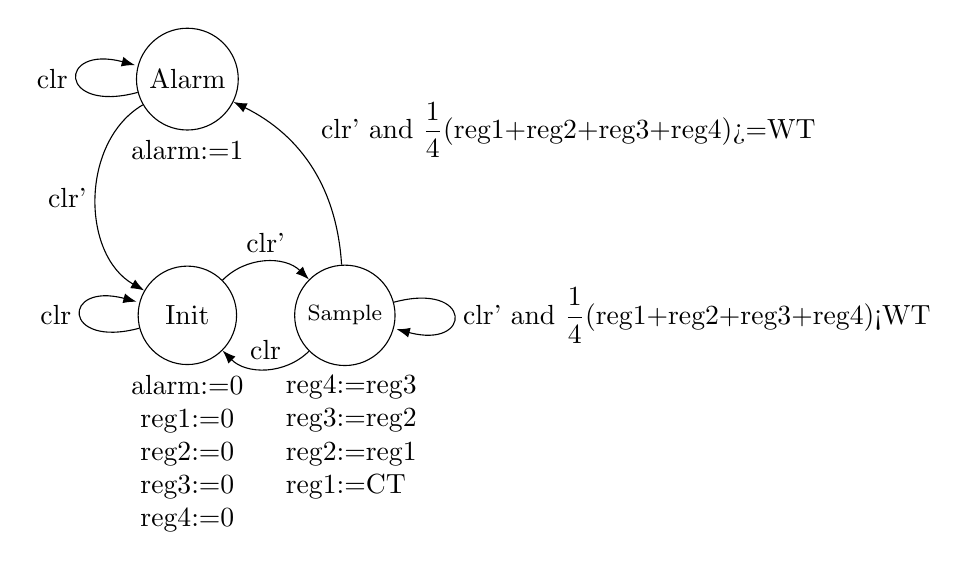
\begin{tikzpicture}[>/.tip={Latex}]
	\draw (0,0) node (init) [draw,shape=circle,minimum size=1.25cm] {Init};
	\node [below,text width=1.5cm,align=center] at (init.south) {alarm:=0 reg1:=0 reg2:=0 reg3:=0 reg4:=0};
	\draw (2,0) node (sample) [draw,shape=circle,minimum size=1.25cm] {\footnotesize Sample};
	\node [below,text width=1.5cm,align=center] at (sample.south) {reg4:=reg3 reg3:=reg2 reg2:=reg1 reg1:=CT };
	\draw (0,3) node (alarm)	 [draw,shape=circle,minimum size=1.25cm] {Alarm};
	\node [below,text width=1.5cm,align=center] at (alarm.south) {alarm:=1};

	\path[->] (init) edge [bend left=45] node [above] {clr'} (sample);
	\path[->] (sample) edge [bend left=45] node [above] {clr} (init);
	\path[->] (sample) edge [loop right] node [right] {clr' and $\dfrac{1}{4}$(reg1+reg2+reg3+reg4)<WT} (w1);
	\path[->] (sample) edge [bend right=30] node [above right] {clr' and $\dfrac{1}{4}$(reg1+reg2+reg3+reg4)>=WT} (alarm);
	\path[->] (alarm) edge [loop left] node {clr} ();
	\path[->] (init) edge [loop left] node {clr} ();
	\path[->] (alarm) edge [bend right=60] node [left] {clr'} (init);
\end{tikzpicture}
\end{center}

Step 2: Datapath Design

\begin{center}
\begin{tikzpicture}
	
	\drawregister{(0,9)}{r1}{32-bit register}{32}
	\drawregister{(0,6)}{r2}{32-bit register}{32}
	\drawregister{(0,3)}{r3}{32-bit register}{32}
	\drawregister{(0,0)}{r4}{32-bit register}{32}

	\drawadder{(4.5,6)}{a1}{32-bit Adder}{32}
	\drawadder{(4.5,0)}{a2}{32-bit Adder}{32}
	\drawadder{(9.5,0)}{a3}{32-bit Adder}{32}
	
	\drawshifter{(4.5,3.5)}{s1}{32-bit $>>$ 1}{32}
	\drawshifter{(4.5,-2.5)}{s2}{32-bit $>>$ 1}{32}
	\drawshifter{(9.5,-2.5)}{s3}{32-bit $>>$ 1}{32}
	
	\drawcmp{(9.5,6)}{lt}{32-bit <}{32}
	
	
	\draw (r1.south)++(down:5mm) -| ($(a1.north)+(left:5mm)$);
	\draw (r2.south)++(down:5mm) -- ++(right:2.5cm) -- ++(up:3.5cm) -| ($(a1.north)+(right:5mm)$);
	\draw (r3.south)++(down:5mm) -| ($(a2.north)+(left:5mm)$);
	\draw (r4.south)++(down:5mm) -- ++(right:2.5cm) -- ++(up:3.5cm) -| ($(a2.north)+(right:5mm)$);
	\draw (s1.south)++(down:5mm) -| ($(a3.north)+(left:5mm)$);
	\draw (s2.south)++(down:5mm) -- ++(right:2.5cm) -- ++(up:5.5cm) -| ($(a3.north)+(right:5mm)$);
	\draw (s3.south)++(down:5mm) -- ++(right:2.5cm) -- ++(up:11.5cm) -| ($(lt.north)+(left:5mm)$);
	
	\filldraw (r1.south)++(down:5mm) circle [radius=0.5mm];
	\filldraw (r2.south)++(down:5mm) circle [radius=0.5mm];
	\filldraw (r3.south)++(down:5mm) circle [radius=0.5mm];
	
	\draw (lt.north) ++(right:5mm) ++(up:2cm) node (WT) {WT};
	\draw (lt.north) ++(right:5mm) -- (WT);
	\draw (lt.south) ++(down:1.5cm) node (avg_lt_wt) {avg\_lt\_wt};
	\draw (lt.south) -- (avg_lt_wt);
	\draw (r1.north) ++(up:1.5cm) node (CT) {CT};
	\draw (r1.north) -- (CT);
	\draw (r1.east) ++(right:2cm) node (clock) {clock};
	\draw (r1.west) ++(up:2.5cm) ++(left:10mm) node (reg_ld) {ld};
	\draw (r1.west) ++(up:2cm) ++(left:5mm) node (reg_clr) {clr};
	\draw (r4.east) -- ++(right:5mm) |- (clock);	
	\draw (r4.west) ++(up:2.5mm) -| (reg_ld);	
	\draw (r4.west) ++(down:2.5mm) -| (reg_clr);	
	\foreach \i in {1,2,3} {
		\draw (r\i.east) -- ++(right:5mm);
		\filldraw (r\i.east) ++(right:5mm) circle [radius=0.5mm];
		\draw (r\i.west) ++(up:2.5mm) -- ++(left:10mm);
		\draw (r\i.west) ++(down:2.5mm) -- ++(left:5mm);
		\filldraw (r\i.west) ++(up:2.5mm) ++(left:10mm) circle [radius=0.5mm];
		\filldraw (r\i.west) ++(down:2.5mm) ++(left:5mm) circle [radius=0.5mm];
	}
\end{tikzpicture}
\end{center}

Step 3: Connect the datapath to a controller

\begin{center}
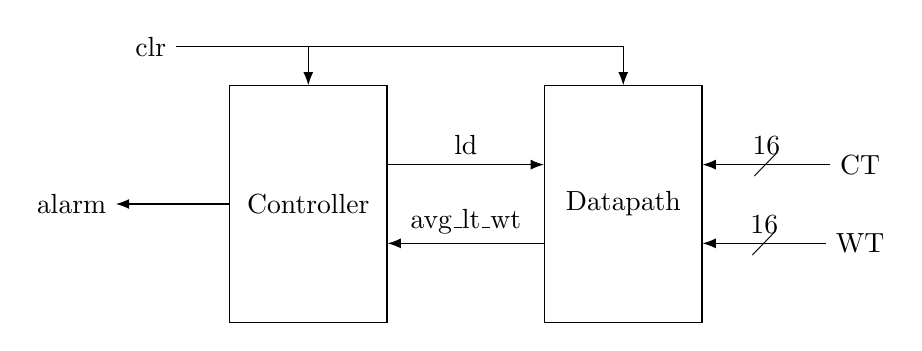
\begin{tikzpicture}[>/.tip={Latex}]
	\draw (-2,0) node (ct) [shape=rectangle,draw,minimum height=3cm,minimum width=2cm] {Controller};
	\draw (2,0) node (dp) [shape=rectangle,draw,minimum height=3cm,minimum width=2cm] {Datapath};
	\draw (-4,2) node (clr) {clr};
	\draw[->] (clr) -| (ct);
	\draw[->] (clr) -| (dp);
	\draw[->] (ct.east) ++(up:5mm) -- node [above] {ld} ($(dp.west)+(up:5mm)$);
	\draw[->] (dp.west) ++(down:5mm) -- node [above] {avg\_lt\_wt} ($(ct.east)+(down:5mm)$);
	\draw (dp.east) ++(up:5mm) ++(right:2cm) node (CT) {CT};
	\draw (dp.east) ++(down:5mm) ++(right:2cm) node (WT) {WT};
	\draw (ct.west) ++(left:2cm) node (alarm) {alarm};
	\draw[->] (CT) -- node {$\diagup$} node [above] {16} ($(dp.east)+(up:5mm)$);
	\draw[->] (WT) -- node {$\diagup$} node [above] {16} ($(dp.east)+(down:5mm)$);
	\draw[->] (ct.west) -- (alarm);
\end{tikzpicture}
\end{center}

Step 4: FSM Design

Inputs: clr

Outputs: alarm

\begin{center}
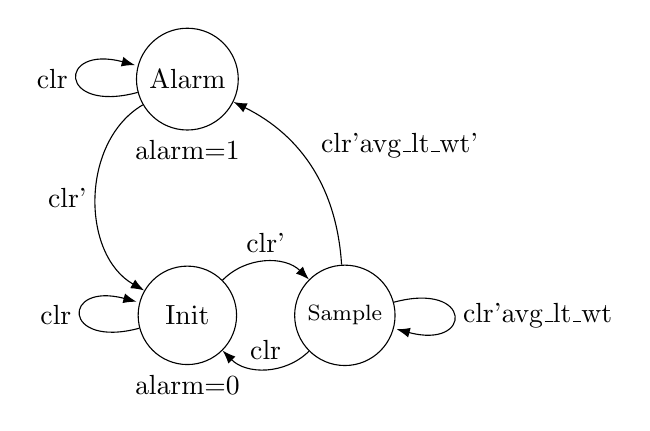
\begin{tikzpicture}[>/.tip={Latex}]
	\draw (0,0) node (init) [draw,shape=circle,minimum size=1.25cm] {Init};
	\node [below,text width=1.5cm,align=center] at (init.south) {alarm=0};
	\draw (2,0) node (sample) [draw,shape=circle,minimum size=1.25cm] {\footnotesize Sample};
	\draw (0,3) node (alarm)	 [draw,shape=circle,minimum size=1.25cm] {Alarm};
	\node [below,text width=1.5cm,align=center] at (alarm.south) {alarm=1};

	\path[->] (init) edge [bend left=45] node [above] {clr'} (sample);
	\path[->] (sample) edge [bend left=45] node [above] {clr} (init);
	\path[->] (sample) edge [loop right] node [right] {clr'avg\_lt\_wt} (w1);
	\path[->] (sample) edge [bend right=30] node [above right] {clr'avg\_lt\_wt'} (alarm);
	\path[->] (alarm) edge [loop left] node {clr} ();
	\path[->] (init) edge [loop left] node {clr} ();
	\path[->] (alarm) edge [bend right=60] node [left] {clr'} (init);
\end{tikzpicture}
\end{center}

\section{}


\end{document}
